\documentclass{article}
\usepackage{graphicx}
\usepackage{amsmath}
\usepackage{booktabs}
\usepackage{siunitx}
\usepackage{float}

\title{Assignment 5 - EE4725 Quasi Optical Systems}
\author{Daniel Tyukov \\ Student Number: 5714699 \\ Microelectronics, TU Delft}
\date{April 2026}

\begin{document}

\maketitle

\tableofcontents
\newpage

%% ====================================================================
\section{System Parameters}
%% ====================================================================

The system under analysis is an infinite planar phased array of printed dipole strips on a rectangular lattice in free space, fed at the centre of every element with a progressive phase taper to scan the beam to $(\theta_0,\phi_0)$. Two unit-cell sizes are studied at a fixed frequency:

\begin{itemize}
\item Operating frequency: $f = \SI{10}{GHz}$, $\lambda_0 = c/f = \SI{30}{mm}$, $k_0 = 2\pi/\lambda_0 = \SI{209.44}{rad/m}$
\item Free-space impedance: $\zeta_0 = 120\pi\;\Omega$
\item Dipole geometry: length $l = \SI{14}{mm}$ ($\approx 0.467\,\lambda_0$, just below first resonance), width $w = \SI{1}{mm}$
\item Lattice case A: $d_x = d_y = \SI{15}{mm}$ ($\lambda_0/2$, sub-half-wave spacing)
\item Lattice case B: $d_x = d_y = \SI{20}{mm}$ ($2\lambda_0/3$, super-half-wave spacing)
\item Floquet truncation: $|m_x|, |m_y| \leq 30$ (Re$\{Z_{in}\}$ is converged exactly at $M=0$ at broadside; Im$\{Z_{in}\}$ converges logarithmically and is within 1\% at $M=30$).
\end{itemize}

The current on each dipole is approximated by a single entire-domain sinusoidal basis function $b(x,y) = i(x)\,j_t(y)$ with
\begin{equation}\label{eq:basis}
i(x) = \frac{\sin\!\big(k_0(l/2 - |x|)\big)}{\sin(k_0 l/2)},\qquad
j_t(y) = \frac{\mathrm{rect}_{[-w/2,\,w/2]}(y)}{w}.
\end{equation}
Their Fourier transforms are
\begin{equation}\label{eq:basis_FT}
I(k_x) = \frac{2k_0\big[\cos(k_x l/2) - \cos(k_0 l/2)\big]}{(k_0^2 - k_x^2)\sin(k_0 l/2)},
\qquad
J_t(k_y) = \mathrm{sinc}\!\left(\frac{k_y w}{2}\right) = \frac{\sin(k_y w/2)}{k_y w/2}.
\end{equation}
The apparent pole of $I(k_x)$ at $k_x = \pm k_0$ is removable; L'H\^opital gives the limit $I(\pm k_0) = l/2$, which is enforced numerically.

%% ====================================================================
\section{Theory: Active Input Impedance via Periodic MoM}
%% ====================================================================

For an infinite array, every element radiates in the presence of all the others. Floquet's theorem reduces the analysis to one unit cell with the periodic boundary condition $\boldsymbol{j}(x+n_x d_x, y+n_y d_y) = \boldsymbol{j}(x,y)\,e^{-jk_{x0}n_x d_x}\,e^{-jk_{y0}n_y d_y}$, where $(k_{x0}, k_{y0}) = (k_0\sin\theta_0\cos\phi_0,\;k_0\sin\theta_0\sin\phi_0)$ is the scan wavenumber. After Galerkin projection of the EFIE on the basis function~\eqref{eq:basis}, the active input impedance is the discrete Floquet sum
\begin{equation}\label{eq:Zactive}
\boxed{\;
Z_{in,\text{active}}(\theta_0,\phi_0) = -\frac{1}{d_x d_y}\sum_{m_x=-\infty}^{\infty}\sum_{m_y=-\infty}^{\infty}
\widetilde{G}_{xx}^{ej}(k_{xm},\,k_{ym})\;\big[I(k_{xm})\big]^2\;\big[J_t(k_{ym})\big]^2\;
}
\end{equation}
with the Floquet wavenumbers
\begin{equation}\label{eq:floquet}
k_{xm} = k_{x0} - \frac{2\pi m_x}{d_x},\qquad
k_{ym} = k_{y0} - \frac{2\pi m_y}{d_y},
\end{equation}
and the spectral free-space dyadic Green's function
\begin{equation}\label{eq:Gxx}
\widetilde{G}_{xx}^{ej}(k_x,k_y) = -\frac{\zeta_0\,(k_0^2 - k_x^2)}{2k_0\,k_z},\qquad
k_z = \begin{cases}\sqrt{k_0^2 - k_x^2 - k_y^2} & \text{(propagating)} \\ -j\sqrt{k_x^2+k_y^2-k_0^2} & \text{(evanescent)}.\end{cases}
\end{equation}

The sum can be split into a propagation contribution and a reactance contribution:
\begin{equation}\label{eq:decomp}
Z_{in,\text{active}} = \underbrace{Z_{00}}_{\text{fundamental, propagating}} + \underbrace{Z_{ho}}_{\text{higher-order, mostly evanescent}}.
\end{equation}
Real power radiates only when a Floquet mode is propagating ($k_{xm}^2 + k_{ym}^2 \leq k_0^2$); evanescent modes store reactive energy near the array.

%% ====================================================================
\section{Q1: Active input impedance vs scan angle}
%% ====================================================================

Equation~\eqref{eq:Zactive} is evaluated at $f = \SI{10}{GHz}$ on a $1441$-point grid $\theta_0 \in [-89^\circ,\,+89^\circ]$ for $\phi_0 = 0^\circ$ (E-plane, dipole-axis plane), $\phi_0 = 90^\circ$ (H-plane, perpendicular plane), and $\phi_0 = 45^\circ$ (D-plane).

\subsection{Broadside reference}

Table~\ref{tab:broadside} compares the broadside ($\theta_0 = 0$) impedance from the full Floquet sum with the closed-form $Z_{00}$ contribution alone.

\begin{table}[H]
\centering
\caption{Broadside active input impedance: full Floquet sum vs.\ fundamental-mode-only formula. The two values of Re$\{Z\}$ agree exactly because all higher-order modes are evanescent at broadside.}
\label{tab:broadside}
\begin{tabular}{@{}lcc@{}}
\toprule
& $d_x = d_y = \SI{15}{mm}$ & $d_x = d_y = \SI{20}{mm}$ \\
\midrule
Floquet sum, $M=30$ & $61.935 - j\,22.788\;\Omega$ & $34.838 - j\,16.385\;\Omega$ \\
$Z_{00}$ analytic   & $61.935\;\Omega$            & $34.838\;\Omega$            \\
\bottomrule
\end{tabular}
\end{table}

The closed-form value is
\begin{equation}\label{eq:Z00}
Z_{00}\big|_{\theta_0=0} = \frac{\zeta_0}{2\,d_x d_y}\cdot\big[I(0)\big]^2,\qquad
I(0) = \frac{2k_0\big(1 - \cos(k_0 l/2)\big)}{k_0^2\,\sin(k_0 l/2)} = 8.60\times10^{-3}\;\text{m},
\end{equation}
which gives $\SI{61.94}{\Omega}$ for the 15-mm cell and $\SI{34.84}{\Omega}$ for the 20-mm cell, matching the simulation to all decimal places. The reactive part ($-j\,22.8\,\Omega$ and $-j\,16.4\,\Omega$) is capacitive because the dipole length $l = 0.467\lambda_0$ is just below resonance.

\subsection{Q1 results}

Figure~\ref{fig:zin_full} shows Re$\{Z_{in}\}$ and Im$\{Z_{in}\}$ for both lattices and all three scan planes; Figure~\ref{fig:zin_mag} plots $|Z_{in}|$ on a log scale to compare singularities at a glance; Figure~\ref{fig:zin_zoom} isolates the H-plane scan-blindness for the 20-mm case.

\begin{figure}[H]
\centering
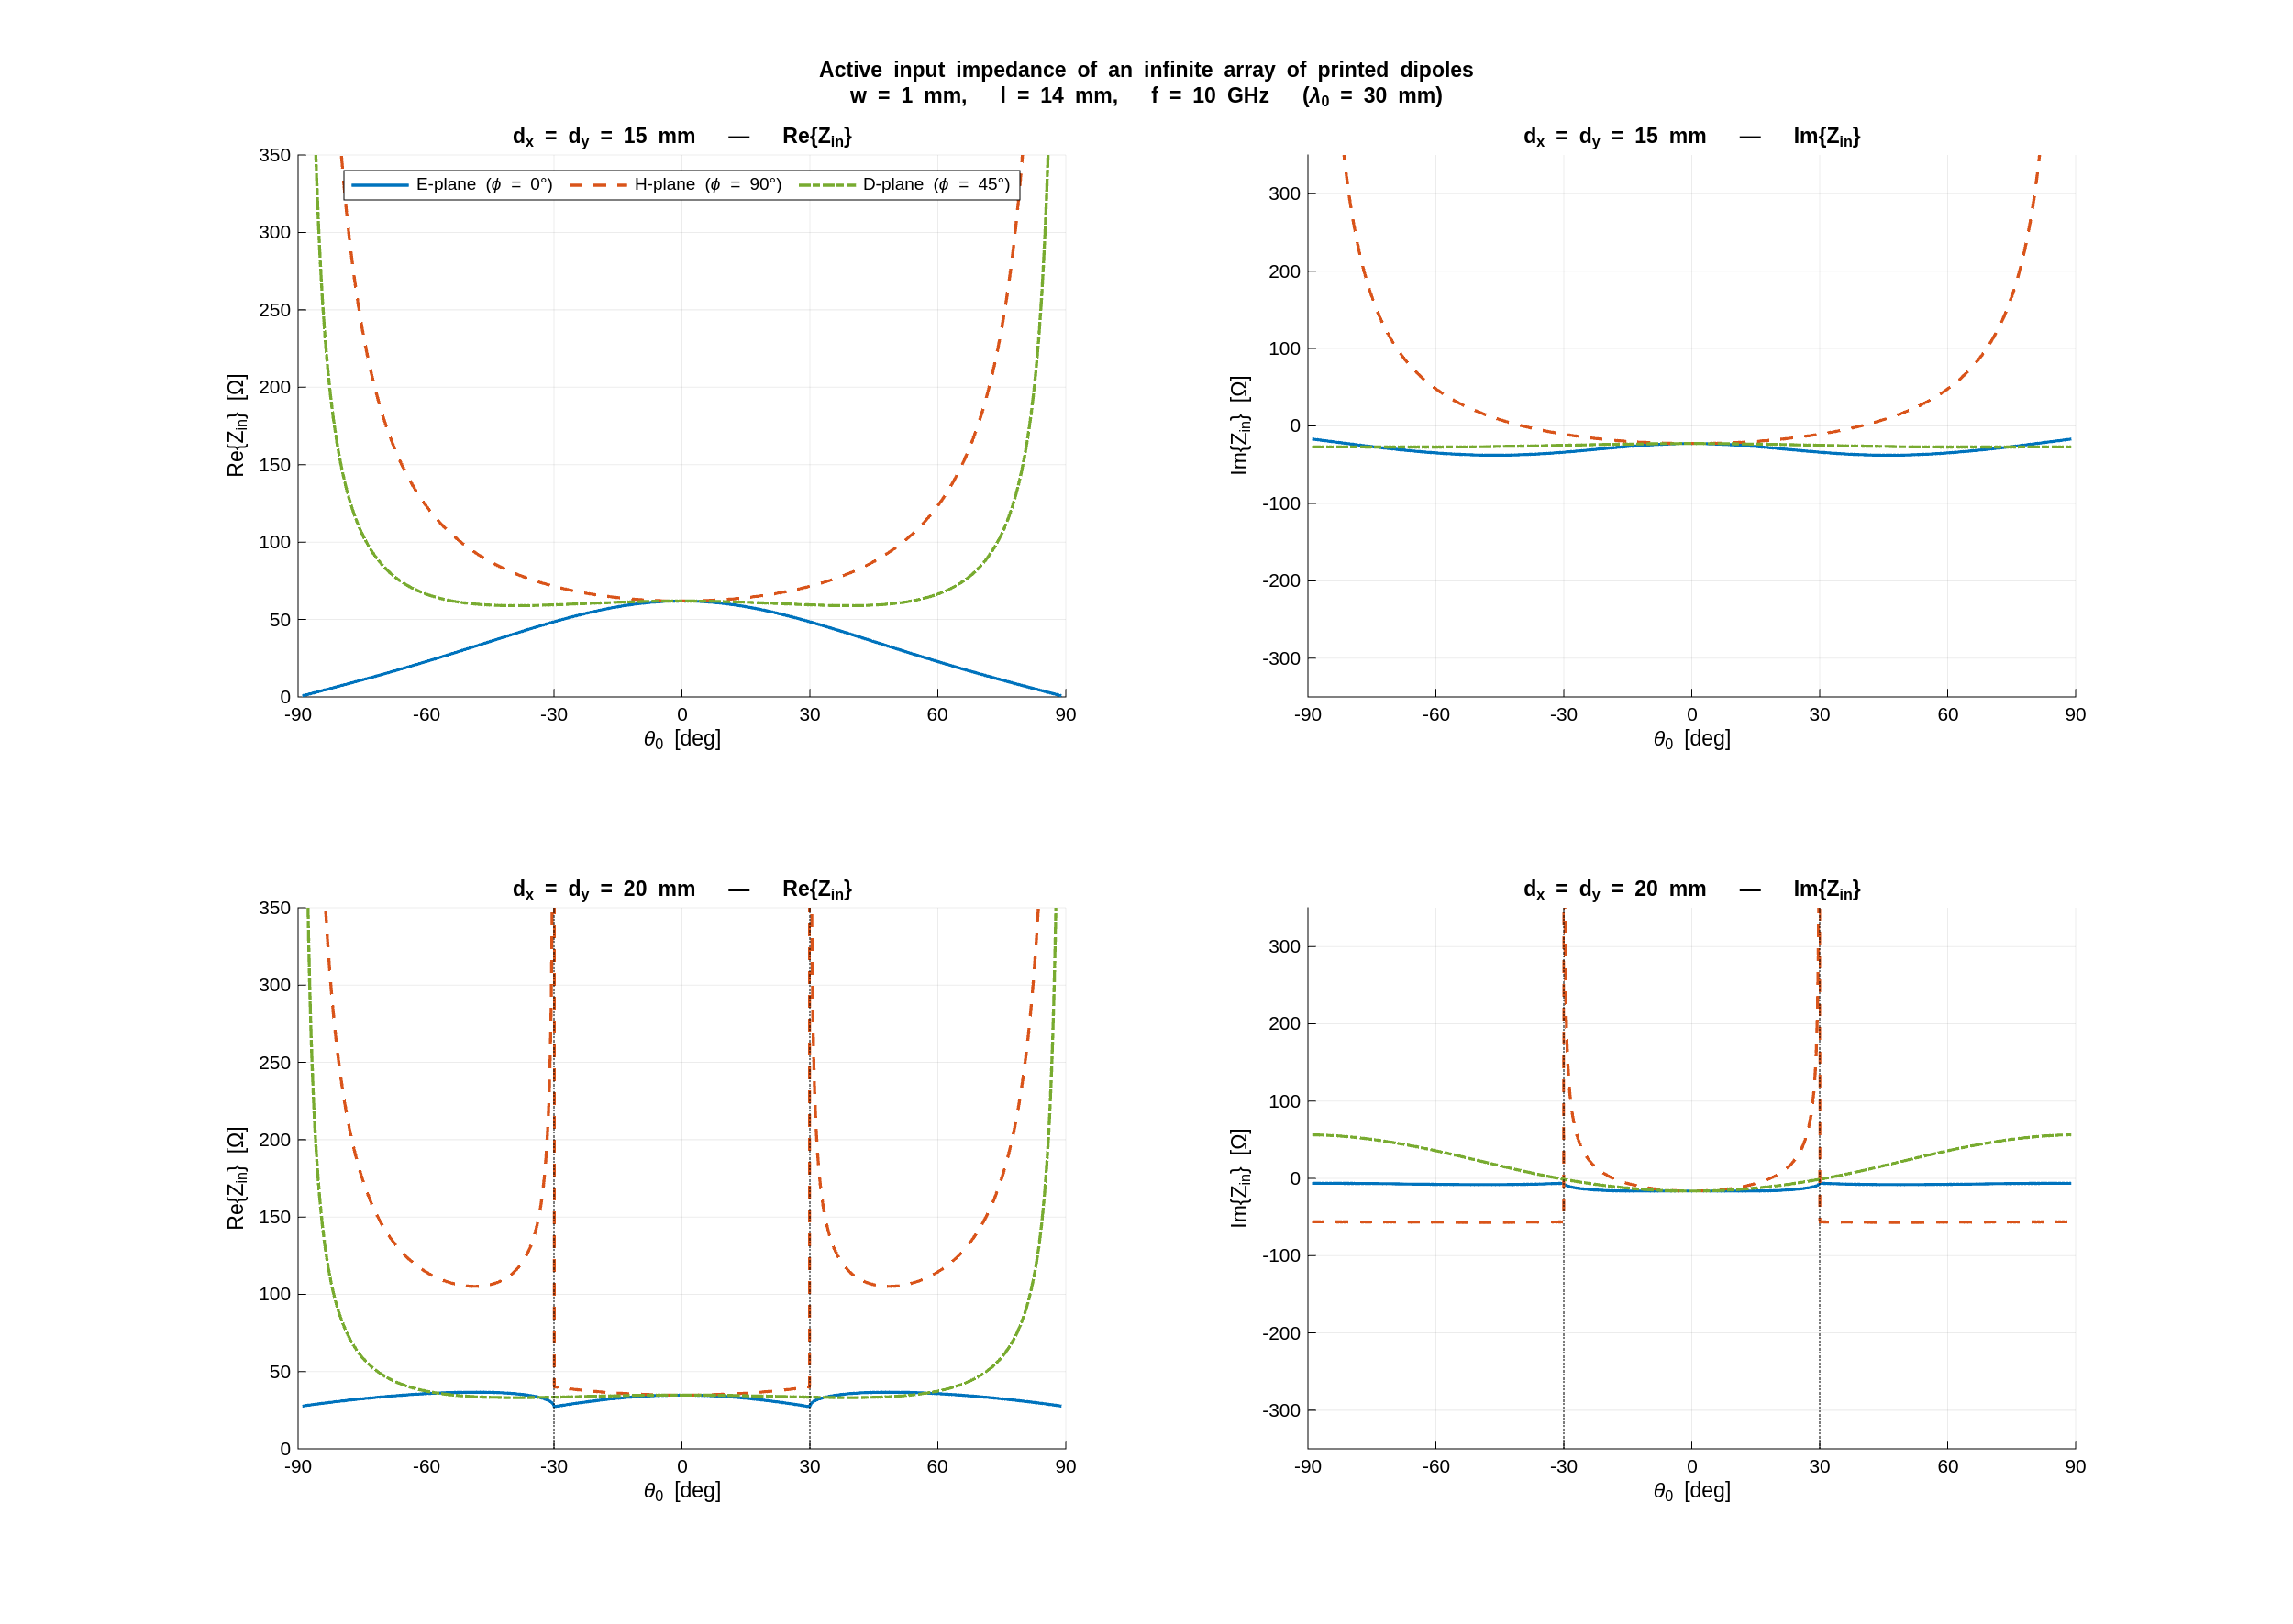
\includegraphics[width=0.95\textwidth]{figures/Q1_Zin_vs_angle.png}
\caption{Active input impedance (resistance and reactance) vs scan angle for the two lattices. The 20-mm lattice (bottom) develops a sharp singularity at $\theta_0 = \pm 30^\circ$ in the H-plane; the 15-mm lattice (top) is smooth across the entire scan range up to endfire.}
\label{fig:zin_full}
\end{figure}

\begin{figure}[H]
\centering
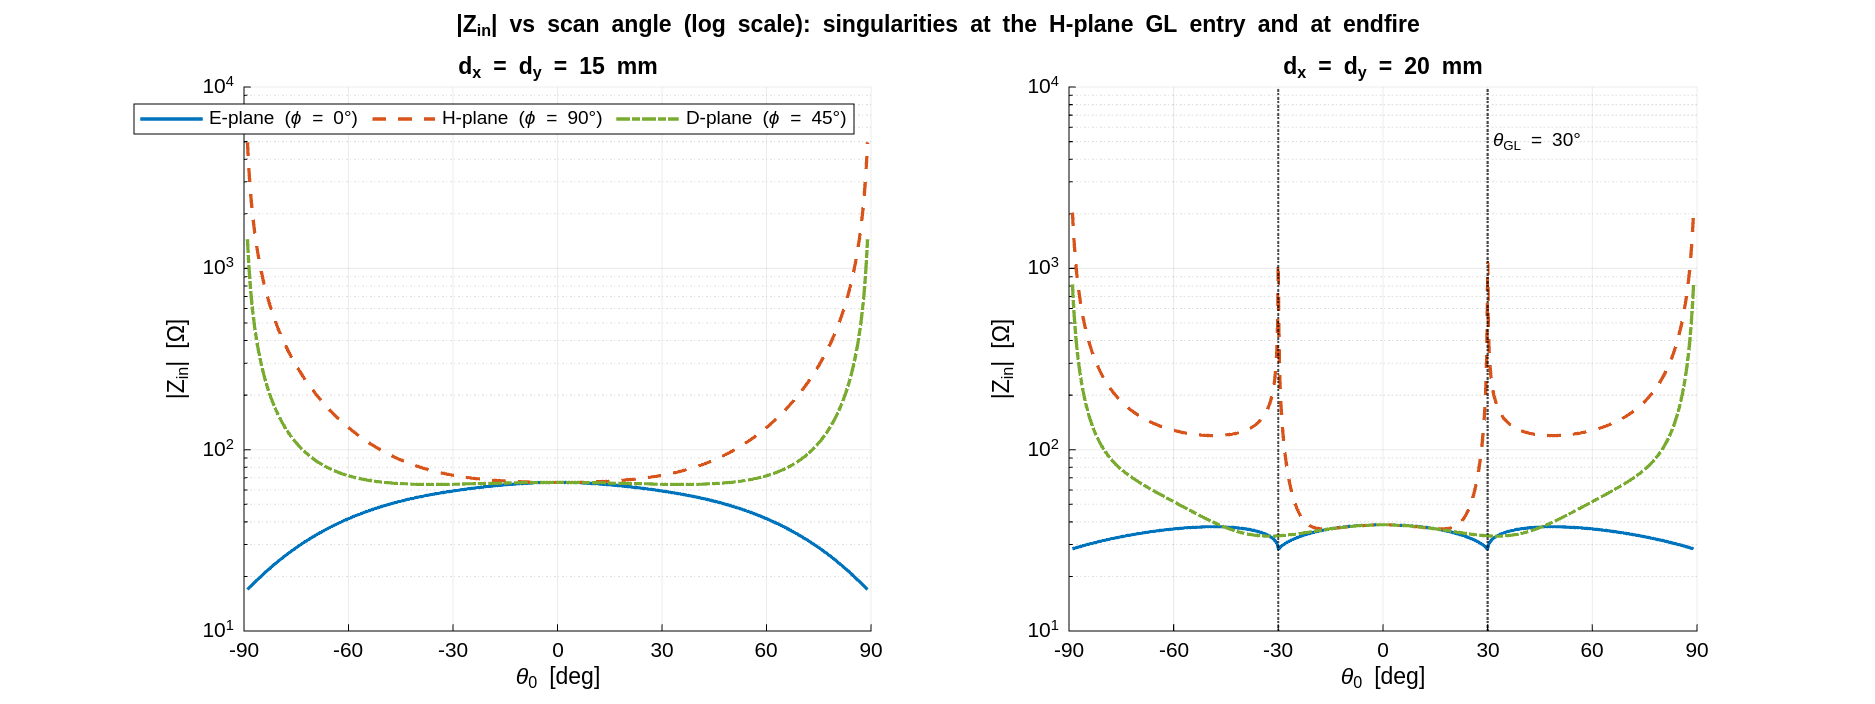
\includegraphics[width=0.95\textwidth]{figures/Q1_Zin_magnitude.png}
\caption{$|Z_{in}|$ on a log scale highlights both the natural endfire singularity (all planes diverge as $\theta_0 \to \pm 90^\circ$, except the E-plane which has the spectral GF zero compensating $1/k_z$) and, for the 20-mm lattice, the H-plane GL singularity at $\theta_0 = \pm 30^\circ$.}
\label{fig:zin_mag}
\end{figure}

\begin{figure}[H]
\centering
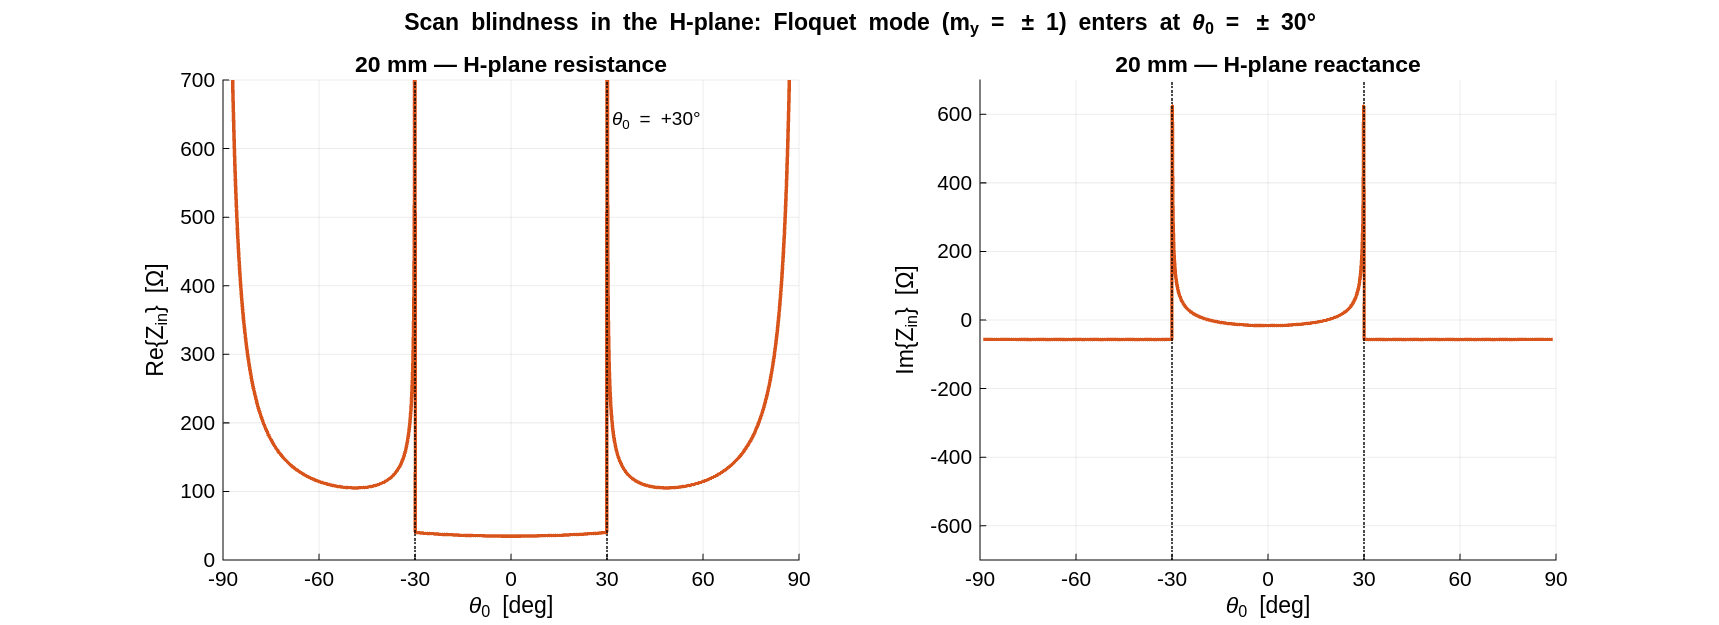
\includegraphics[width=0.95\textwidth]{figures/Q1_Zin_zoom_Hplane_20mm.png}
\caption{Detail of the 20-mm H-plane impedance. As $\theta_0$ approaches $30^\circ$ from below, the $(m_x=0, m_y=\pm 1)$ Floquet mode is evanescent and contributes a strong inductive reactance (Im$\{Z_{in}\} \to +\infty$). Just above $30^\circ$ that mode propagates: Re$\{Z_{in}\}$ jumps from $\SI{40}{\Omega}$ to $\sim\SI{2}{k\Omega}$ before settling around $\SI{100}{\Omega}$. Both Re$\{Z\}$ and Im$\{Z\}$ show one-sided $1/\sqrt{|\theta - \theta_{GL}|}$ divergences.}
\label{fig:zin_zoom}
\end{figure}

\subsection{Why the impedance changes with angle in the E and H planes}

In the \textbf{E-plane} ($\phi_0 = 0^\circ$, $k_{y0} = 0$), the scan moves the spectral observation point along $\hat{x}$. The fundamental-mode Green's function evaluated on the scan trajectory is
\begin{equation}
\widetilde{G}_{xx}^{ej}(k_{x0}, 0) = -\frac{\zeta_0\,(k_0^2 - k_{x0}^2)}{2k_0\,k_{z0}} = -\frac{\zeta_0}{2k_0}\,\sqrt{k_0^2 - k_{x0}^2} = -\frac{\zeta_0}{2}\cos\theta_0,
\end{equation}
so $\mathrm{Re}\{Z_{00}\} \propto \cos\theta_0$ and the resistance \emph{decreases} smoothly with the E-plane scan angle. The dipole projects most of its current onto the propagating plane wave at broadside, and that projection drops as $\cos\theta_0$ as the wave tilts away from $\hat{z}$. This matches the blue curve in Figure~\ref{fig:zin_full}.

In the \textbf{H-plane} ($\phi_0 = 90^\circ$, $k_{x0} = 0$), the fundamental-mode Green's function is
\begin{equation}
\widetilde{G}_{xx}^{ej}(0, k_{y0}) = -\frac{\zeta_0\,k_0^2}{2k_0\,k_{z0}} = -\frac{\zeta_0\,k_0}{2k_0\cos\theta_0} = -\frac{\zeta_0}{2\cos\theta_0},
\end{equation}
so $\mathrm{Re}\{Z_{00}\} \propto 1/\cos\theta_0$ and the resistance \emph{increases} with the H-plane scan angle. The dipole still presents its full transverse cross-section to the wave, but the impedance of the propagating Floquet mode itself increases as the wave tilts. This explains the rising H-plane curve in Figure~\ref{fig:zin_full}.

The opposite trends in the two planes are a direct consequence of the dipole orientation: the $\hat{x}$-directed current radiates a $\hat{\theta}$-polarised field whose projection along $\hat{\theta}$ varies as $\cos\theta_0$ in the E-plane and as $1$ in the H-plane, while the modal wave impedance carries the $1/\cos\theta_0$ factor that shows up only in the H-plane.

The \textbf{D-plane} sits between the two: $\widetilde{G}_{xx}^{ej}(k_0\sin\theta_0/\sqrt{2}, k_0\sin\theta_0/\sqrt{2}) = -\zeta_0(k_0^2 - k_0^2 \sin^2\theta_0/2)/(2k_0 k_{z0})$, which combines an E-plane-like numerator factor and an H-plane-like $1/k_{z0}$ factor and lies between the two trends.

\subsection{Singularities in the active input impedance}

Two distinct types of singularity appear in $Z_{in,\text{active}}$:

\begin{enumerate}
\item \textbf{Fundamental endfire singularity} ($\theta_0 \to \pm 90^\circ$). The fundamental Floquet wavenumber $k_{z0} = k_0\cos\theta_0$ approaches zero, so the modal impedance diverges and any antenna over an infinite ground (or in any infinite array) cannot radiate strictly endfire. This singularity exists for every lattice and every plane, and is purely geometric---it is not caused by the periodicity of the array. In the E-plane it is masked by the compensating zero of the numerator $(k_0^2 - k_{x0}^2)$, so the E-plane Re$\{Z\}$ stays bounded there.

\item \textbf{Higher-order Floquet (Wood/Rayleigh) singularity}. For the 20-mm lattice, the $(m_x=0, m_y=\pm 1)$ mode crosses the visible region boundary at exactly $\theta_0 = \pm 30^\circ$ in the H-plane: as $\theta_0 \to 30^\circ$ from below, $k_{z,(0,\pm 1)} = \sqrt{k_0^2 - k_{ym}^2} \to 0$ on the evanescent side, and as $\theta_0$ exceeds $30^\circ$ the same mode is propagating. The Green's function factor $1/k_{z,(0,\pm 1)}$ produces a one-sided $1/\sqrt{|\theta_0 - \theta_{GL}|}$ divergence: the reactance blows up to $+\infty$ on the evanescent side and the resistance blows up to $+\infty$ on the propagating side. After the threshold, the mode carries propagating power and the resistance settles at an elevated level (about $\SI{100}{\Omega}$ vs $\SI{40}{\Omega}$ before threshold). This is the textbook \emph{scan-blindness} behaviour and is what makes super-half-wave lattices unusable past $\theta_{GL}$.
\end{enumerate}

The \textbf{E-plane} of the 20-mm lattice does \emph{not} show this divergence (Figure~\ref{fig:zin_mag}, blue curve, has only a small dip at $\pm 30^\circ$). The reason is that in the E-plane the grating-lobe candidate is $(m_x=\pm 1, m_y=0)$, for which both $k_{xm}^2 \to k_0^2$ and the numerator factor $(k_0^2 - k_{xm}^2) \to 0$ at threshold. Since $\widetilde{G}_{xx}^{ej} \propto (k_0^2 - k_{xm}^2)/k_{zm}$ and $k_{zm} \propto \sqrt{k_0^2 - k_{xm}^2}$ near threshold, the ratio actually goes to zero. Physically, the dipole current is parallel to the propagation direction of the E-plane grating lobe, so it cannot couple to it---the grating lobe is forbidden by polarisation. In the H-plane the grating lobe is broadside-polarised relative to the dipole, so the coupling is maximal and the singularity is fully exposed.

For the 15-mm lattice ($\lambda_0/d = 2$) all higher-order Floquet circles only \emph{touch} the visible region at endfire, so no scan-blindness singularity appears anywhere within $|\theta_0| < 90^\circ$ (Figure~\ref{fig:zin_full}, top row).

%% ====================================================================
\section{Q2: Grating-lobe diagrams}
%% ====================================================================

The propagation condition $k_{xm}^2 + k_{ym}^2 \leq k_0^2$ in normalised wavenumber coordinates $u = k_{x0}/k_0 = \sin\theta_0\cos\phi_0$, $v = k_{y0}/k_0 = \sin\theta_0\sin\phi_0$ becomes
\begin{equation}\label{eq:gldiag}
\left(u - \frac{\lambda_0\,m_x}{d_x}\right)^2 + \left(v - \frac{\lambda_0\,m_y}{d_y}\right)^2 \leq 1.
\end{equation}
The visible region is the unit circle $u^2 + v^2 \leq 1$. A Floquet mode $(m_x, m_y)$ propagates when the unit circle of radius $1$ centred on $(\lambda_0 m_x/d_x,\,\lambda_0 m_y/d_y)$ overlaps the visible region. Figure~\ref{fig:gl_diag} plots these circles for both lattices together with the three scan trajectories.

\begin{figure}[H]
\centering
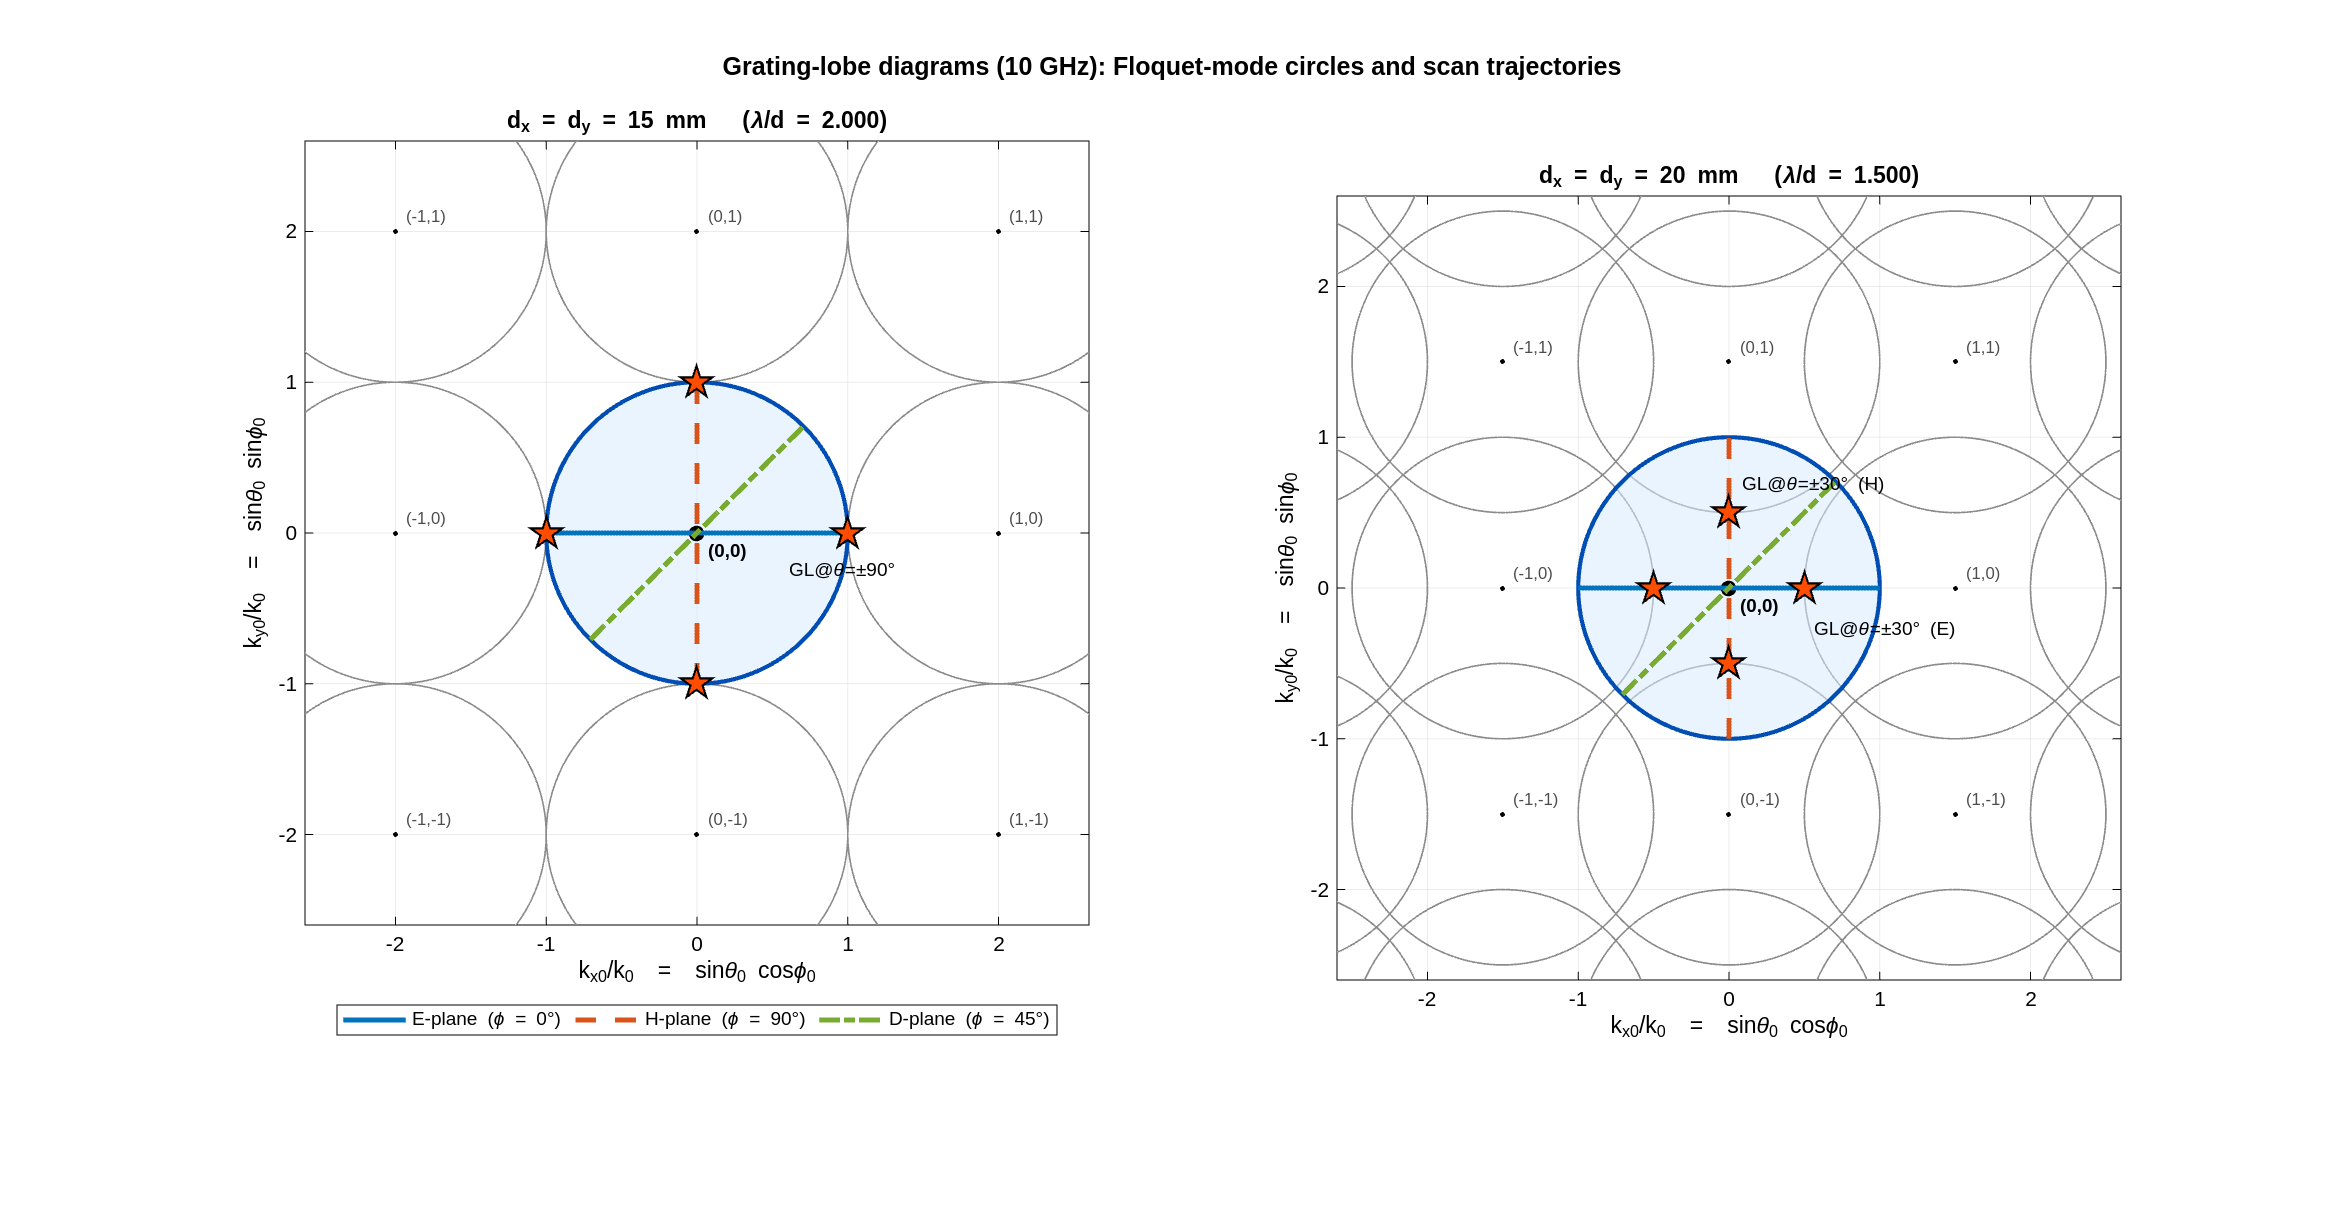
\includegraphics[width=\textwidth]{figures/Q2_grating_lobe_diagram.png}
\caption{Grating-lobe diagrams. The blue disc is the visible region (fundamental mode). Grey circles are the higher-order Floquet circles. \textbf{Left:} 15-mm lattice ($\lambda_0/d = 2$), the higher-order circles only touch the visible region at endfire---no grating lobes inside $|\theta_0|<90^\circ$. \textbf{Right:} 20-mm lattice ($\lambda_0/d = 1.5$), the four nearest higher-order circles overlap the visible region; the red stars mark where the E- and H-plane scan trajectories first enter another Floquet circle, both at $\theta_0 = \pm 30^\circ$. The D-plane (green dash-dot) misses every higher-order circle, as confirmed by the smooth Im$\{Z\}$ in Figure~\ref{fig:zin_full}.}
\label{fig:gl_diag}
\end{figure}

\begin{table}[H]
\centering
\caption{Grating-lobe entry angles (10 GHz). For the 15-mm lattice the GL circles only touch at endfire; for the 20-mm lattice they enter at exactly $\pm 30^\circ$ in the principal planes and never along the diagonal.}
\label{tab:gl}
\begin{tabular}{@{}lccc@{}}
\toprule
Lattice & E-plane $(\phi=0^\circ)$ & H-plane $(\phi=90^\circ)$ & D-plane $(\phi=45^\circ)$ \\
\midrule
$d = \SI{15}{mm}$ & $\theta_{GL} = 90^\circ$ (touch only) & $90^\circ$ (touch only)        & none (misses) \\
$d = \SI{20}{mm}$ & $\theta_{GL} = 30.00^\circ$            & $30.00^\circ$ \emph{(scan blindness)} & none (misses) \\
\bottomrule
\end{tabular}
\end{table}

\subsection{Mode entries by plane}

\textbf{E-plane scan} ($u \neq 0$, $v = 0$). The trajectory along the $u$-axis enters the $(m_x = +1, m_y = 0)$ circle (centred at $(\lambda_0/d, 0)$) at $u = \lambda_0/d - 1$:
\begin{itemize}
\item 15-mm lattice: $u_{GL} = 2 - 1 = 1$, so $\theta_{GL} = 90^\circ$ (touch at endfire only).
\item 20-mm lattice: $u_{GL} = 1.5 - 1 = 0.5$, so $\theta_{GL} = \arcsin(0.5) = 30^\circ$.
\end{itemize}
By the polarisation argument above, the impedance change at this E-plane GL entry is a knee, not a divergence---the mode contributes zero net coupling at threshold.

\textbf{H-plane scan} ($u = 0$, $v \neq 0$). Same algebra with $d_y$: the $(0, \pm 1)$ mode enters at $v_{GL} = \lambda_0/d_y - 1$. Same $\theta_{GL}$ as in the E-plane (since $d_x = d_y$), but the impedance now diverges because the dipole is fully cross-polarised relative to the grating lobe.

\textbf{D-plane scan} ($u = v = \sin\theta_0/\sqrt{2}$). For the closest higher-order circle $(m_x = -1, m_y = 0)$ centred at $(-\lambda_0/d, 0)$, equation~\eqref{eq:gldiag} becomes
\begin{equation}
\left(\sin\theta_0/\sqrt{2} + \lambda_0/d\right)^2 + \sin^2\theta_0/2 \leq 1
\;\Leftrightarrow\;
\sin^2\theta_0 + \sqrt{2}\,(\lambda_0/d)\sin\theta_0 + (\lambda_0/d)^2 - 1 \leq 0.
\end{equation}
The discriminant is $2(\lambda_0/d)^2 - 4\big[(\lambda_0/d)^2 - 1\big] = 4 - 2(\lambda_0/d)^2$, which is negative for both lattices ($-4$ for 15 mm, $-0.5$ for 20 mm). Hence the D-plane trajectory \emph{never} enters any first-order Floquet circle---only the natural endfire singularity affects the diagonal scan. The stronger 2D periodicity of the lattice is partly defeated by scanning along the diagonal because the scan trajectory threads between the higher-order centres.

%% ====================================================================
\section{Summary}
%% ====================================================================

\begin{itemize}
\item The active input impedance of the dipole array was computed via the Floquet-mode sum~\eqref{eq:Zactive} truncated at $|m_x|, |m_y| \leq 30$. Re$\{Z\}$ at broadside is exact at $M=0$ ($\SI{61.93}{\Omega}$ at 15 mm, $\SI{34.84}{\Omega}$ at 20 mm); Im$\{Z\}$ is converged to $<1\%$ at $M=30$.
\item The E-plane and H-plane impedance trends with scan angle are opposite by construction: the E-plane resistance decreases as $\cos\theta_0$ (current projection drops with the wave tilt), the H-plane resistance increases as $1/\cos\theta_0$ (the modal wave impedance grows). The D-plane sits between the two.
\item Two singularity types appear: (i) the natural endfire singularity at $\theta_0 = \pm 90^\circ$, common to all lattices, and (ii) the Wood/Rayleigh grating-lobe singularity, which appears \emph{only} in the H-plane of the 20-mm lattice at $\theta_0 = \pm 30^\circ$. The E-plane of the same lattice has its grating-lobe coupling killed by polarisation.
\item The grating-lobe diagrams confirm the scan-angle predictions exactly: $\sin\theta_{GL} = \lambda_0/d - 1$ in the principal planes ($90^\circ$ for 15 mm, $30^\circ$ for 20 mm), and no first-order GL ever enters along the diagonal at either lattice. The 15-mm lattice is the standard $\lambda_0/2$ design choice for grating-lobe-free phased-array operation; the 20-mm lattice is unusable beyond $\theta_0 = 30^\circ$ in the H-plane and is the textbook example of scan blindness.
\end{itemize}

\end{document}
